\chapter{Mappatura}\label{chap:mapping}

\section{Il modello per RDF}

L'analisi preliminare ha inizialmente considerato lo specifico sottoinsieme di 113 campi utilizzati dalla Fondazione Zeri, assieme ai campi specifici aggiunti da quest'ultima.\\
Il modello della Scheda F è incredibilmente dettagliato e ricco di informazioni ma ``piatto'': manca perciò di flessibilità nel realizzare collegamenti tra le diverse entità, richiedendo riferimenti ad Authority File o vocabolari controllati per diversi campi e risultando particolarmente vulnerabile a errori ortografici e di inserimento.

Dal momento che l'obiettivo era quello di portare l'archivio fotografico Zeri nel dominio LOD, viste anche le precedenti esperienze (vedi \ref{sec:towards-a-new-model}), CIDOC-CRM è stato scelto come miglior standard in modo da aumentarne al massimo la fruibilità.

L'effettiva mappatura è stata necessariamente sottoposta ad alcuni compromessi, data la natura estremamente flessibile di CIDOC-CRM: lo standard è infatti pensato per coprire una gran varietà di casi, dai musei alle biblioteche, e manca quindi di alcune specificità tipiche di un modello qual è la Scheda F, che essendo disegnato per la fotografia arrichisce in maniera peculiare.

Lo sforzo è stato comunque quello di estendere il meno possibile CIDOC-CRM così da rimanere aderenti allo standard quanto più si è riusciti.

Dal momento che l'obiettivo era rendere disponibile i dati della Scheda F in un triple store, quindi RDF, il linguaggio che è risultato ovvio utilizzare è OWL 2 DL (\cite{8}). Tutto il materiale utilizzato per lo sviluppo della F Entry Ontology (FEO) (secondo la metodologia \emph{SAMOD - Simplified Agile Methodology for Ontology Development\footnote{\url{http://www.essepuntato.it/samod}}}) è già disponibile online\footnote{\url{http://www.essepuntato.it/2014/03/fentry/samod}}, così come la versione attuale dell'ontologia \emph{F Entry Ontology}\footnote{\url{http://www.essepuntato.it/2014/03/fentry}}.

\subsection{L'ontologia F Entry Ontology}\label{sec:feo}
La versione attuale di FEO introduce le classi e le proprietà che caratterizzano i tre concetti fondamentali: la fotografia, l'opera d'arte che ne è soggetto e la stessa Scheda F che descrive la fotografia e il suo soggetto.

La Scheda F è un documento che contiene metadati che descrivono una fotografia che ha per soggetto un'opera d'arte fisica (o un suo particolare) o un gruppo di opere d'arte. Sebbene nella collezione sia presente una sola copia per ogni Scheda F, esistono per la stessa fotografia diverse versioni, e per la stessa opera d'arte sono possibili più fotografie; inoltre la stessa opera d'arte può essere stata sottoposta a trasformazioni ritratte nel tempo da diverse fotografie.

Per registrare correttamente tale complessità di relazioni e caratterizzazioni dipendenti da tempo e contesto dell'entità, la Scheda F, la fotografia e l'opera d'arte sono state descritte e categorizzate concettualmente secondo i termini di Functional Requirements for Bibliographic Recors (FRBR), come segue:
\begin{description}
\item[La Scheda F] contiene dati riguardo la stessa catalogazione, quelli riguardanti la rappresentazione ricadono nel livello \emph{Work} di FRBR e quelli riguardo la sua collocazione ricadono nel livello \emph{Item}.
\item[La fotografia] registra uno specifico evento fotografico in uno specifico momento ma può essere presente in diverse forme nella collezione (e.g. positivo/negativo, diversi tipi di stampa, etc\ldots) e per ogni forma possono esistere copie multiple, ognuna con la propria storia; per questo l'essenza della fotografia è rappresentata dal livello \emph{Work} di FRBR, ogni forma di questa fotografia diventa \emph{Manifestation} e ogni copia individuale ricade nel livello \emph{Item}.
\item[L'opera d'arte] è un oggetto fisico potenzialmente sottoposto a diversi eventi di trasformazione (deterioramenti, restauri, etc\ldots); perciò l'essenza dell'opera d'arte è rappresentata dal livello \emph{Work} di FRBR, il risultato di ogni traformazione dal livello \emph{Manifestation} e le sue caratteristiche fisiche dal livello \emph{Item}.
\end{description}

Tali caratterizzazioni sono soggette ad attribuzione autoriale come risultato di un'attività di produzione che coinvolge degli agenti in uno specifico momento nel tempo.\\
Per modellare questi aspetti sono state importate alcune ontologie preesistenti:
\begin{description}\label{sec:imported-ontologies}
\item[FaBiO - FRBR-aligned Bibliographic Ontology] \cite{6} è un'ontologia basata su FRBR originariamente sviluppata per registrare descrizioni di entità bibliografiche pubblicate o potenzialmente pubblicabili, oppure entità che sono collegate da riferimenti bibliografici, o ancora entità utilizzate per definire questi ultimi. Le entità in FaBiO sono principalmente pubblicazioni testuali quali libri, riviste, giornali e elementi di contenuto quali articoli, relazioni di conferenza e editoriali; oltre a questi descrivono anche blog, pagine web, dataset, algoritmi, immagini, metadati di documenti, protocolli sperimentali, specifiche formali e vocabolari, pezze legali, governative, report tecnici e commeciali e pubblicazioni simili e infine antologie, cataloghi e altre collezioni.
\item[PROV-O - Provenance Ontology] \cite{18} offre un set di classi, proprietà e limiti utilizzabili per rappresentare le informazioni di provenienza riguardo le attività (e.g. la creazione di una fotografia), gli agenti coinvolti (e.g. l'autore della fotografia, il venditore e il compratore in una transazione) e le entità che produce (e.g. il dipinto, la Scheda F, la fotografia).
\end{description}

La versione attuale di FEO è stata strutturata in base alle necessità di descrivere concettualmente e fisicamente la scheda, l'oggetto fotografico e l'oggetto fotografato; una panoramica delle principali classi e relazioni dell'ontologia è visibile in fig.~\ref{fig:feo-mainclasses}.

\begin{figure}
    \centering
    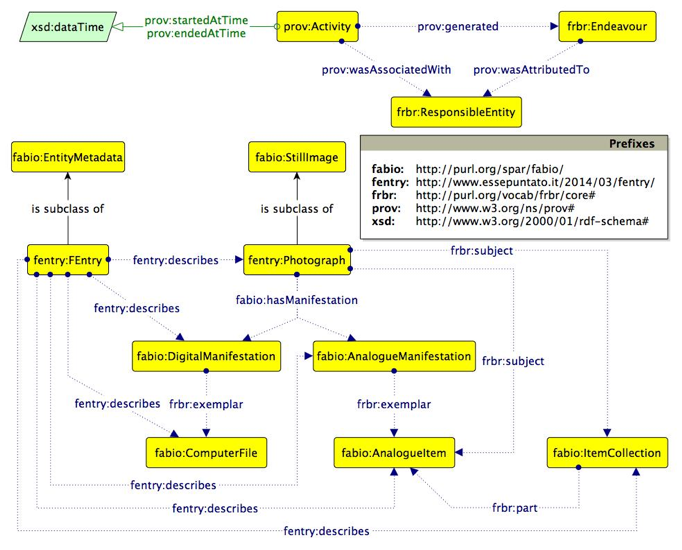
\includegraphics[width=100mm]{images/feo-mainclasses.png}
	\caption{Le relazioni e classi principali definite in FEO - diagramma Graffoo (\protect\url{http://www.essepuntato.it/graffoo})}
	\label{fig:feo-mainclasses}
\end{figure}

Il modello di FEO usa diverse entità descritte in ontologie esterne, principalmente \emph{PROV-O} \cite{22} (prefisso \emph{prov}), la versione OWL 2 DL di FRBR\footnote{\url{http://purl.org/spar/frbr}} (prefisso \emph{frbr}) e \emph{FaBiO} \cite{6} (prefisso \emph{fabio}).

Uno dei concetti principali dell'ontologia è la Scheda F, definita come un particolare documento contenente metadati circa una fotografia e l'oggetto reale rappresentato da quest'ultima. Viene descritta in termini di Work FRBR (i.e. la classe \emph{fentry:FEntry} sottoclasse di \emph{fabio:EntityMetadata}) e di Item FRBR (come file digitale disponibile online, i.e. la classe \emph{fabio:ComputerFile}). La proprietà \emph{fentry:describes} collega istanze di \emph{fentry:FEntry} alle istanze di tutte le altre classi (a prescindere dal livello FRBR), tra le quali \emph{fentry:Photograph}, \emph{fabio:ArtisticWork}, etc\ldots

La fotografia è definita come rappresentazione visuale e statica di un dato oggetto reale (o parte di esso, o di un gruppo di oggetti reali); è descritta come Work FRBR (i.e. la classe \emph{fentry:Photograph} sottoclasse di \emph{fabio:StillImage}), Manifestation FRBR (i.e. le classi \emph{fabio:DigitalManifestation} e \emph{fabio:AnalogueManifestation}) e Item FRBR (i.e. le classi \emph{fabio:ComputerFile} e \emph{fabio:AnalogueItem}). La proprietà \emph{frbr:subject} collega la fotografia all'oggetto reale rappresentato.

L'oggetto reale rappresentato da una fotografia è descritto in termini di Work FRBR (i.e. la classe \emph{fabio:ArtisticWork}), Manifestation FRBR (i.e. la classe \emph{fabio:AnalogueManifestation}) e Item FRBR (la classe \emph{fabio:AnalogueItem}).

\section{La mappatura}
Nel modello della Scheda F è evidente come la divisione in paragrafi la sezioni in parti semanticamente indipendenti e afferenti ad uno specifico concetto FRBR (Work, Expression, Manifestation, Item); ciò permette di procedere alla mappatura affrontando i paragrafi come blocchi unitari, sezioni logiche che coinvolgono un numero limitato di entità legate ai dati documentati nei campi del modello stesso.

In fase di definizione è stato fatto tesoro di tutte le esperienze finora descritte assieme ad alcune più specifiche (e.g. \cite{12}).

La mappatura completa realizzata è visibile in tab. \ref{tab:schedaf-to-owl}; di seguito sono riassunte le principali classi utilizzate per rappresentare le singole entità. Sono tralasciati i livelli FRBR visti in \ref{sec:feo}, concentrandosi invece sulla mappatura in classi CIDOC-CRM (prefisso \emph{crm}).

\subsection{Oggetto fotografico e Scheda F}
Il modella della Scheda F riguarda la descrizione delle fotografie le quali sono, dal punto di vista di CIDOC-CRM, oggetti fisici creati dall'uomo, quindi la classe designata per la rappresentazione è naturalmente \emph{crm:E22 Man-Made Object}. La stessa Scheda F è rappresentata dalla classe \emph{crm:E31 Document} legata alla fotografia dalla proprietà \emph{crm:P70 documents}.

Dal momento che le fotografie dell'archivio Zeri hanno tutte come soggeto una certa opera d'arte, la Scheda F è legata alla relativa Scheda OA, anch'essa istanza di \emph{crm:E31 Document}, tramite la proprietà \emph{crm:P67 refers to}.

\subsection{Livello Work}

L'opera d'arte risulta essere, in CIDOC-CRM, un oggetto fisico creato dall'uomo e pertanto descritto (come la fotografia) tramite la classe \emph{E22 Man-Made Object} e legata alla fotografia dalla proprietà \emph{P62 is depicted by}.

L'autore della fotografia può essere un individuo (e.g. Federico Zeri) o un ente (e.g. Magnum Photo Agency), pertanto per la rappresentazione non è possibile nella gerarchia di classi di CIDOC-CRM oltre alla classe \emph{E39 Actor}, legato alla fotografia dall'attività e dal ruolo caratteristico che ha avuto: e.g. l'autore principale è collegato tramite la proprietù \emph{crm:P14 performed} all'attività di produzione descritta come istanza di \emph{E12 Production}, quest'ultima a sua volta legata alla fotografia dalla proprietà \emph{crm:P108 has produced}; autori alternativi e produttori sono legati in maniera simile con l'aggiunta, nel caso sia presente, del ruolo avuto nella produzione della fotografia, descritto con la classe \emph{pro:roleInTime} fornita dalla Publishing Roles Ontology - PRO\footnote{\url{http://purl.org/spar/pro}}.

\subsection{Livello Manifestation}

Dal punto di vista di FRBR la descrizione dell'oggetto ricade nel livello Manifestation; qui vengono documentate alcune caratteristiche specifiche dell'oggetto stesso, quali:
\begin{description}
\item[Materiali] dei quali è composto l'oggetto, descritte con la classe \emph{crm:E57 Material} e collegate con la proprietà \emph{crm:P45 consist of}.
\item[Dimensioni] ovvero altezza, larghezza, spessore, diametro: sebbene nella Scheda F siano sezionate in campi ad hoc, CIDOC-CRM non dispone di tale specificità, offrendo una generica classe \emph{crm:E54 Dimension} ulteriormente dettagliata con le proprietà \emph{crm:P2 has type}, \emph{crm:P90 has value} e \emph{crm:P91 has unit}; le dimensioni così istanziate vengono poi legate all'oggetto dalla proprietà \emph{crm:P43 has dimension}\footnote{e.g. photo (E22) \emph{has dimension (P43)} height of photo (E54) \emph{has type (P2)} height (E62), \emph{has unit (P91)} mm (E58), \emph{has value (P90)} 227 (E60)}.
\item[Tecnica] usata nella produzione della fotografia, è rappresentata come istanza di \emph{crm:E55 Type} collegata a \emph{crm:E12 Production} tramite la proprietà \emph{crm:P32 used technique}; l'istanza di \emph{crm:E12 Production} è a sua volta collegata alla fotografia tramite la proprietà \emph{crm:P108 was produced by}. Nel particolare caso delle tecniche e più in generale tutte le volte in cui viene utilizzata come classe descrittiva \emph{crm:E55 Type}, la scelta del tipo è mappata in vocabolari controllati da ICCD o analoghi tesauri.
\end{description}

Oltre ai dati riguardanti l'oggetto fisico, il modello della Scheda F permette al catalogatore di aggiungere alla creazione della foto delle informazioni cronologiche e spaziali sul luogo dello scatto. Dal momento che tale creazione riguarda comunque l'oggetto, ricade anch'essa nel livello Manifestation. Le classi scelte per rappresentare gli eventi di creazione e produzione sono \emph{crm:E65 Creation} e \emph{crm:E12 Production} legati all'oggetto rispettivamente dalle proprietà \emph{crm:P94 was created by} e \emph{crm:P108 was produced by} e a loro volta legate ad una istanza di \emph{crm:E53 Place} tramite la proprietà \emph{crm:P7 took place at} per le indicazioni spaziali e ad un'istanza di \emph{crm:P4 Period} tramite \emph{crm:P10 falls within} per le indicazioni cronologiche.

Altri dati d'interesse riguardanti il livello Manifestation sono il tipo dell'oggetto (e.g. positivo, negativo, stampa, etc\dots) naturalmente rappresentato da un'istanza di \emph{E55 Type} che mappa il vocabolario controllato di ICCD e legato all'oggetto tramite \emph{crm:P2 has type}; il numero di oggetti fisici che compongono l'oggetto stesso, rappresentati da un'istanza di \emph{crm:E60 Number} legata con \emph{crm:P57 has number of parts}.

Le possibili relazioni con altri oggetti fotografici (de-composizione per fotografie complesse o correlate) sono descritte nel modello della Scheda F con l'indicazione della raccolta superiore e sono pertanto state rappresentate come collegamento via \emph{crm:P46 forms part of} all'istanza specifica di \emph{E18 Physical Thing}.

Infine, anche le indicazioni di copyright ricadono nel livello Manifestation e sono state descritte con la classe \emph{crm:E30 Right} legata all'oggetto fotografico tramite la proprietà \emph{crm:P104 is subject to}\footnote{il dominio della proprietà \emph{P104} è la classe \emph{crm:E72 Legal Object}, il collegamento è tuttavia legittimo grazie al fatto che la classe \emph{crm:E22 Man-Made Object} deriva sia da \emph{crm:E71 Man-Made Thing} che da \emph{crm:E72 Legal Object}}.

\subsection{Livello Item}

Il modello della Scheda F include alcuni campi per documentare la posizione attuale (geografica e archivistica) dell'oggetto fotografico ed eventuali posizioni precedenti. In CIDOC-CRM tali posizioni sono descritte tramite la classe \emph{crm:E53 Place}, anche quelle archivistiche (e.g. inventario e collocazione). Per definire la posizione attuale dell'oggetto è stata scelta la proprietà \emph{crm:P54 has current permanent location} mentre per le precedenti posizioni la proprietà è \emph{crm:P53 has former or current location}.

Nel definire le coordinate temporali di queste ultime è stata sfruttata la \emph{Time Ontology in OWL}\footnote{\url{http://www.w3.org/TR/owl-time/}} che offre delle primitive particolari (i.e. \emph{time:Istant}, \emph{time:hasBeginning} e \emph{time:hasEnd}) per specificare ulteriormente la blanda precisione della classe \emph{crm:E52 Time-Span} di CIDOC-CRM. Tali coordinate temporali sono state applicate (con \emph{crm:P4 has time-span}) ad un'istanza di \emph{crm:E9 Move} legata a sua volta all'oggetto fotografico tramite la proprietà \emph{crm:P25 moved}.

Eventuali posizioni annidate (e.g. la collocazione all'interno di un edificio posizionato geograficamente oppure la busta all'interno di un fascicolo) sono state collegate tra di loro tramite la proprietà \emph{crm:P89 falls within}.

Le condizioni fisiche e lo stato di conservazione riguardano altresì il livello Item. Tali informazioni sono state descritte con la classe \emph{crm:E3 Condition State} e legate all'oggetto con la proprietà \emph{crm:P44 has condition}. Dal momento che lo stato di conservazione è definito in un vocabolario controllato, le varie tipologie sono state mappate in istanze di \emph{crm:E55 Type} e legate alla condizione tramite \emph{crm:P2 has type}.

\subsection{Proprietà della Scheda F}

Le proprietà della Scheda F stessa consistono principalmente di dati amministrativi, il più importante dei quali è l'identificatore interno al catalogo, descritto con la classe \emph{crm:E42 Identifier} tramite la proprietà \emph{crm:P48 has preferred identifier}.

Il tipo di scheda identifica il modello all'interno di quelli forniti da ICCD, nel caso specifico è dunque sempre uguale a ``F'' ed è descritto tramite \emph{crm:E55 Type} e relativa proprietà \emph{crm:P2 has type}.

L'istituto o ente responsabile della conservazione, non potendo fare assunzioni specifiche sulla sua natura, è descritto come istanza di \emph{crm:E40 Legal Body} e legato alla scheda tramite la proprietà \emph{crm:P50 has current keeper}.

Ulteriori dati vengono registrati per:
\begin{itemize}
\item il catalogatore che ha creato la prima versione della scheda, istanza di \emph{crm:E39 Actor}, legato all'istanza di \emph{crm:E65 Creation} tramite \emph{crm:P14 carried out by} e quest'ultima a sua volta legata all'oggetto scheda da \emph{crm:P94 created}; le coordinate temporali sulla catalogazione sono descritte tramite la classe \emph{crm:E52 Time-Span} e legate all'attività di creazione con \emph{crm:P4 has time-span}.
\item gli aggiornamenti effettuati sulla catalogazione, analoghi alla catalogazione ma descritti tramite un'istanza di \emph{crm:E81 Trasformation} in luogo di \emph{crm:E65 Creation}.
\end{itemize}
